\PID
Отпорност NTC термистора у функцији температуре дата је изразом у облику\footnote{Природна експоненцијална функција је
$\exp x = \ee^x$, где је $\ee$ Ојлеров број, основа природног логаритма.} 
${R(T) = R_0 \exp\left(\upbeta\left( \dfrac1T - \dfrac1{T_0} \right) \right)}$, \vspace{1mm} при чему су 
$R_0 = 10\unit{k\Omega}$ отпорност при температури ${T_0 = 298\unit{K}}$, док је 
$\upbeta = 3950\unit{K}$. Мерењем је утврђено да је отпорност термистора $R = 1,5\unit{k\Omega}$. Израчунати 
температуру термистора.

\RESENJE 

Задатак представља решавање нелинеарне једначине у аналитички задатом облику. Решавање ове једначине се не може спровести аналитички па 
је потребно применити неки од нумеричких поступака. У овом случају, илустроваћемо примену итеративног Њутн-Рафсоновог метода сечице.
У општем случају тражимо решење једначине облика $f(x) = 0$, низом погађања $x_0$, $x_1$, \ldots, $x_n$ све док се не постигне задовољавајућа
тачност. \vspace{1mm}

\begin{slikaDesno}{fig/nr.pdf}
    Процес започиње иницијалним погађањем $x_0$. Након тога, повлачи се тангента на функцију $f(x)$ у тој тачки, 
    и одређује се пресек тангенте са $x$-осом, чиме се добија вредност $x_1$. Поступак се итеративно понавља чиме 
    низ ${x_i}$ конвергира према правој нули функције $x^\ast$, као што је илустровано на слици. Аналитички облик одређивања 
    наредног корака из претходног може се утврдити на основу осенченог троугла са исте слике. Нагиб хипотенузе тог 
    троугла је по дефиницији извода $f'(x_1) = \dfrac{\Delta y}{\Delta x} = \dfrac{f(x_1)}{x_1 - x_2}$, па је одатле 
    $x_2 = x_1 - \dfrac{f(x_1)}{f'(x_1)}$. 
\end{slikaDesno}

Уопштењем наведеног поступка, прелазак из $i$-тог корака у $(i+1)$-ви корак је онда дат изразом 
\begin{equation}
    x_{i+1} = x_i - \dfrac{f(x_i)}{f'(x_i)}.
\end{equation}
Итерације се израчунавају све док не постане довољно мало $|f(x_i)|$, или док је постане довољно мали прираштај наредног 
корака $|x_i - x_{i-1}| = |f(x_i)/f'(x_i)|$. Проблем конвергенције овог метода се овде неће разматрати. 
У случају овог задатка, може се писати да је 
\begin{equation}
    f(T) = R - R_0 \exp\left(\upbeta\left( \dfrac1T - \dfrac1{T_0} \right) \right),
\end{equation}
па је одговарајући извод 
\begin{equation}
    f'(T) = \dfrac{\de f}{\de T} =  \dfrac{\upbeta R_0}{T^2} \exp\left(\upbeta\left( \dfrac1T - \dfrac1{T_0} \right) \right)
\end{equation}.
Погађање се може започети од прозвољне вредности $T_0$, па се за то може узети и параметар $T_0$ из формулације
задатка. Итеративним израчунавањем се добијају резултати из табеле \ref{tab:\ID:iter}, док је кретање погађања 
по графику $f(T)$ приказано на слици \ref{fig:\ID:iter}. Коначно, закључујемо да је тражена температура
$T \approx 347,6\unit{K}$. Примећује се да метод веома брзо конвергира, па је у свега четири итерације 
пришао веома близу тачног решења. 

\noindent
\begin{minipage}[c]{0.5\textwidth}
    %\begin{table}[ht!]
    \centering
    \begin{tabular}{cccc}
        $i$ & $T_i\unit{[K]}$ & $f(T_i)\unit{[k\Omega/K]}$ & $f'(T_i)\unit{[k\Omega/K^2]}$ \\ \hline
        $0$ & $298,0$ & $-8,50$ & $0,445$ \\
        $1$ & $317,1$ & $-3,00$ & $0,177$ \\
        $2$ & $334,1$ & $-0,89$ & $0,085$ \\
        $3$ & $344,6$ & $-0,17$ & $0,055$ \\
        $4$ & $\boxed{347,6}$ & $-0,01$ & $0,049$ \\
    \end{tabular}
    \captionof{table}{Приказ итерација}
    \label{tab:\ID:iter}
\end{minipage}
%
\begin{minipage}[c]{0.45\textwidth}
    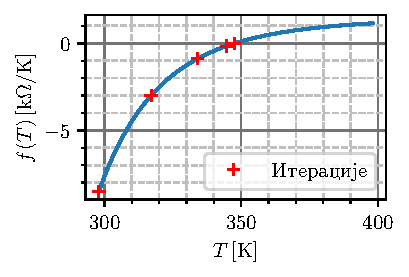
\includegraphics{fig/nr_iter.pdf}
    \captionof{figure}{Графички приказ итерација}
    \label{fig:\ID:iter}
\end{minipage}

